%%%%%%%%%%%%%%%%%%%%%%%%%%%%%%%%%%%%%%%%%
%
% CMPT 435
% Lab Zero
%
%%%%%%%%%%%%%%%%%%%%%%%%%%%%%%%%%%%%%%%%%

%%%%%%%%%%%%%%%%%%%%%%%%%%%%%%%%%%%%%%%%%
% Short Sectioned Assignment
% LaTeX Template
% Version 1.0 (5/5/12)
%
% This template has been downloaded from: http://www.LaTeXTemplates.com
% Original author: % Frits Wenneker (http://www.howtotex.com)
% License: CC BY-NC-SA 3.0 (http://creativecommons.org/licenses/by-nc-sa/3.0/)
% Modified by Alan G. Labouseur  - alan@labouseur.com
%
%%%%%%%%%%%%%%%%%%%%%%%%%%%%%%%%%%%%%%%%%

%----------------------------------------------------------------------------------------
%	PACKAGES AND OTHER DOCUMENT CONFIGURATIONS
%----------------------------------------------------------------------------------------

\documentclass[letterpaper, 10pt]{article} 

\usepackage[english]{babel} % English language/hyphenation
\usepackage{graphicx}
\usepackage{xcolor}
\graphicspath{ {./images/} }
\usepackage[lined,linesnumbered,commentsnumbered]{algorithm2e}
\usepackage{listings}

% Lstlistings configuration
\definecolor{codegreen}{rgb}{0,0.6,0}
\definecolor{codegray}{rgb}{0.5,0.5,0.5}
\definecolor{codepurple}{rgb}{0.58,0,0.82}
\definecolor{backcolour}{rgb}{0.95,0.95,0.92}

\lstdefinestyle{mystyle}{
    backgroundcolor=\color{backcolour},   
    commentstyle=\color{codegreen},
    keywordstyle=\color{magenta},
    numberstyle=\tiny\color{codegray},
    stringstyle=\color{codepurple},
    basicstyle=\ttfamily\footnotesize,
    breakatwhitespace=false,         
    breaklines=true,                 
    captionpos=b,                    
    keepspaces=true,                 
    numbers=left,                    
    numbersep=5pt,                  
    showspaces=false,                
    showstringspaces=false,
    showtabs=false,                  
    tabsize=2
}

\lstset{style=mystyle}
\lstset{language=Java}

\usepackage{fancyhdr} % Custom headers and footers
\pagestyle{fancyplain} % Makes all pages in the document conform to the custom headers and footers
\usepackage{lastpage}
\usepackage{wasysym}
\usepackage{url}

% Set up for minted package. It had some bugs so I decided to only keep lstlistings.
% \usepackage{minted}
% \makeatletter
% \newlength\minted@belowskip
% \define@key{minted@opt}{belowskip}[\@topsepadd]
% {\setlength{\minted@belowskip}{#1}}

% \def\minted@endparenv{%
%   \addpenalty\@endparpenalty\addvspace\minted@belowskip\@endpetrue}
% \def\FV@EndList{%
%   \FV@ListProcessLastLine
%   \FV@EndListFrame
%   \minted@endparenv
%   \endgroup
%   \@endpetrue}
% \makeatother
% \newminted{java}{linenos=true, belowskip=3cm}

\fancyhead{} % No page header - if you want one, create it in the same way as the footers below
\fancyfoot[L]{} % Empty left footer
\fancyfoot[C]{page \thepage\ of \pageref{LastPage}} % Page numbering for center footer
\fancyfoot[R]{}

\renewcommand{\headrulewidth}{0pt} % Remove header underlines
\renewcommand{\footrulewidth}{0pt} % Remove footer underlines
\setlength{\headheight}{13.6pt} % Customize the height of the header

%----------------------------------------------------------------------------------------
%	TITLE SECTION
%----------------------------------------------------------------------------------------

\newcommand{\horrule}[1]{\rule{\linewidth}{#1}} % Create horizontal rule command with 1 argument of height

\title{	
   \normalfont \normalsize 
   \textsc{CMPT 435 - Fall 2021 - Dr. Labouseur} \\[10pt] % Header stuff.
   \horrule{0.5pt} \\[0.25cm] 	% Top horizontal rule
   \huge Assignment Two -- Sorting Algorithms \\     	    % Assignment title
   \horrule{0.5pt} \\[0.25cm] 	% Bottom horizontal rule
}

\author{Augusto Gonzalez-Bonorino \\ \normalsize augusto.gonzalezbonorino1@marist.edu}

\date{\normalsize\today} 	% Today's date.

\begin{document}

\maketitle % Print the title

%----------------------------------------------------------------------------------------
%   CONTENT SECTION
%----------------------------------------------------------------------------------------

% - -- -  - -- -  - -- -  -

\section{Description of the program}
The program aims to implement, and compare, the following sorting algorithms: Insertion, Selection, Merge and Quick sort. In regards to my implementation in Java I have decided to define one MainGonzalezBonorino class which contains the functions necessary to read the input text document containing the Strings to sort and the functions needed to implement each algorithm.The characteristics and details of each algorithm will be explored in detail throughout this documentation


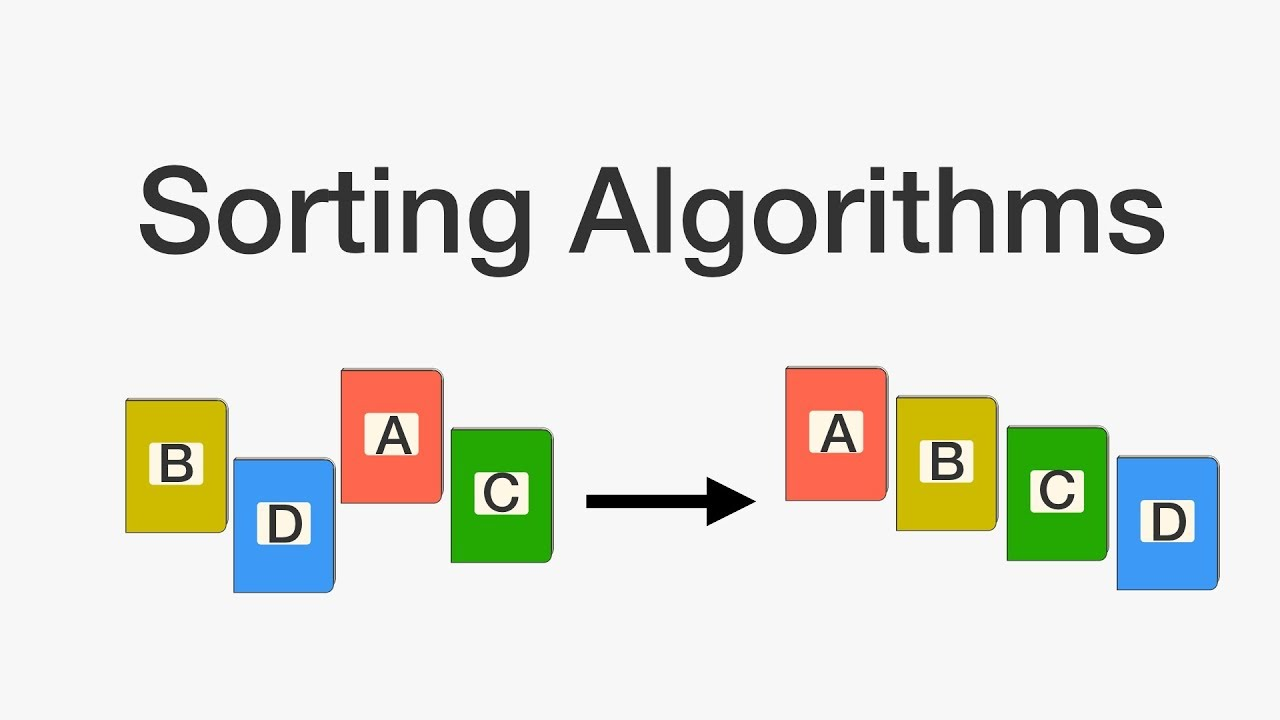
\includegraphics[scale=0.25]{images/sorting_algorithms.jpg}

\pagebreak
\section{Selection Sort}

Selection sort runs in $O(n^2)$ and it works as follows: It repeatedly finds the minimum element of an unsorted section of the array and places that element at the beginning, thereby maintaining two sub arrays (one sorted and one being sorted) until the whole array is traversed. In each iteration the minimum element is moved to the sorted sub array. 

\begin{lstlisting}
public static int selectionSort(String[] magicList) {
		
		knuthShuffle(magicList);
		int len = magicList.length;
		int numComparisons = 0;
		
		for (int i = 0; i < len - 1; i++) {
			
			int smallPos = i;
			
			for (int j = i + 1; j <= len - 1; j++) {
				
				if (magicList[j].compareToIgnoreCase(magicList[smallPos]) < 0 ) //compare strings
				{	
					smallPos = j;
				}
				numComparisons++;
						
			} // inner for loop
			
			// swap
			String temp = magicList[smallPos];
			magicList[smallPos] = magicList[i];
			magicList[i] = temp;
			
		} // outer for loop
		
		return numComparisons;
		
	} // selectionSort
\end{lstlisting}

The java implementation is fairly straightforward. First, to ensure the input array is shuffled, I implement a Knuth shuffle (a.k.a. the Fisher-Yates shuffle) which is commonly used to shuffle arrays. You will soon note that this function is used before implementing each sorting algorithm to make sure that we are not feeding the algorithm an already sorted array. Next, in the outer loop, we instantiate an integer called \textit{smallPos} to keep track of the index of the smallest element. Then, we use that index to loop over each String in the magicitems.txt file and compare them. If, after the comparison was made, one of them was smaller than the current smallest element then \textit{smallPos} is updated and the number of comparisons is incremented. Once we compared the elements, we swap them to create the sorted array. The algorithm repeats the aforementioned steps until the whole array is sorted.
\pagebreak
\section{Insertion Sort}

Insertion sort, like Selection, has a run time of $O(n^2)$. Nevertheless, this algorithm provides an improvement over Selection sort because it avoids looping over the array if a subset of it is already sorted, thereby saving us some precious resources. Therefore, while the worst-case scenario is $O(n^2)$ it is possible to reduce it to $O(n)$ if the array is already sorted. The algorithm divides the array into two sub arrays (sorted and unsorted). Then, values from the unsorted part are picked and placed at the correct position in the sorted part.

\begin{lstlisting}
public static int insertionSort(String[] magicList) {
		
		knuthShuffle(magicList);
		int len = magicList.length;
		int numComparisons = 0;
		
		for (int j = 1; j <= len - 2; j++) {
			
			String key = magicList[j];
			int i = j - 1;
			
			while ( (i >= 0) && ( magicList[i].compareToIgnoreCase(key) > 0) ) {
				
				magicList[i + 1] = magicList[i];
				i = i - 1;
				
				numComparisons++;
				
			} // while loop
			
			magicList[i + 1] = key;
			
		} // for loop
		
		return numComparisons;
		
	} // insertionSort
\end{lstlisting}

After shuffling the input array of Strings we assign the first element to a variable I have called \textit{key}. Then, we compare the current element \textit{key} with the one that precedes it, which is located at index \textit{i}. If the key element is smaller than its predecessor, the program compares it to the previous elements and moves the greater elements one position up to make space for the swapped element. Finally, the current smallest element is inserted into the sorted array. The algorithm repeats these steps until the array is fully sorted.

\pagebreak
\section{Merge Sort}


\end{document}